% !TeX spellcheck = cs_CZ
%{\tikzset{external/prefix={tikz/MAI/}}
% \tikzset{external/figure name/.add={ch10_}{}}
%---------------------------------------------------------------------------------------------------
% file ppst.tex
%---------------------------------------------------------------------------------------------------
\chapter{Počet Pravděpodobnosti}
\minitoc
  Slovo pravděpodobnost používáme velmi často. Jaký však je jeho přesný význam? Jsme přesvědčeni, 
  že pravděpodobnost výhry ve sportce je velmi malá. Ani pravděpodobnost, že se vyplní předpověď 
  počasí, nepovažujeme mnohdy za výraznou. Přesto je mezi oběma příklady obrovský kvantitativní 
  rozdíl. Zkusme význam pojmu pravděpodobnost ukázat pomocí konkrétních číselných příkladů.
  
  \begin{itemize}
    \item \textbf{Příklad se střelcem}: Sportovní střelec střílí na terč série \num{100} ran. 
          Předpokládejme, že podmínky při střelbě jsou stále stejné. Stejná je zbraň, terč, 
          vzdálenost, povětrnostní podmínky i momentální zdravotní stav střelce Při hodnocení 
          střelcova „mistrovství“ někdo řekne, že střelec zasáhne terč s pravděpodobností 
          \num{92}\%. Jak tomu rozumět? Znamená to, že v souboru sérií výstřelů jsou velmi časté 
          ty, v nichž zasáhl střelec terč \num{92}-krát. Samozřejmě, není řídké, že se objeví i 
          série s \num{93} nebo \num{94} zásahy, ale také s \num{91} nebo \num{90}. Vyloučen není 
          ani případ s úspěšností \num{96} či \num{88}, a dokonce i stovku bychom mohli zaznamenat. 
          Situace výrazně odlišné od \num{92} zásahů však budou řídké, a to tím více, čím více se 
          úspěšnost série liší od \num{92} oběma směry.
    \item \textbf{Příklad se zmetky}: Koupíte si výrobek u firmy, o které je známo, že vyrábí 
          zmetky s pravděpodobností 0,16\%? Situaci lze posuzovat obdobně jako úspěšnost střelce. 
          Budeme-li například zkoumat série obsahující 1000 výrobků, bude každá z nich obsahovat „v 
          průměru“ 16\% zmetků. Z příkladu se střelcem již zhruba víme, jak posuzovat slovo v 
          průměru.
  \end{itemize}
  
  V této kapitole se budeme pravděpodobnostmi zabývat podrobněji. Zjistíme, že i když se týkají 
  náhodných jevů, platí i pro ně jisté zákonitosti.
    
  \section{Pravděpodobnost}
    V úvodních příkladech jsme si vyložili, jak intuitivně chápat pojem pravděpodobnost. Jednalo se 
    v nich o posouzení průměrné úspěšnosti ve velkém souboru operací či úkonů prováděných za 
    stejných podmínek, šlo tedy o jakousi „průměrnou“ pravděpodobnost. Nyní definujeme 
    pravděpodobnost matematicky.
    
    \subsection{Co se pravdě podobá — definice pravděpodobnosti}
      Pro definici pravděpodobnosti použijeme pojmu \emph{náhodný pokus}, jehož význam si ukážeme 
      na příkladu. Dobrým příkladem náhodných pokusů je třeba házení mincí, hraní kostkou, výběr 
      karet z balíčku, vidíme-li pouze jejich rub, apod. Budeme třeba házet kostkou. Abychom si 
      situaci zbytečně nekomplikovali, budeme předpokládat, že všechny výsledky hodu kostkou 
      (náhodné pokusy) jsou stejně časté, žádný z nich není nijak preferován\footnote{Kostka by 
      tedy měla být homogenní, plocha, na kterou po hodu dopadne, vodorovná, kvalita povrchu všech 
      stěn kostky stejná (žádná stěna by třeba neměla být natřena lepidlem), apod.}. Počet možných 
      výsledků jednotlivého hodu je \(N = 6\) (kostka má \num{6} stěn, na každé je vyznačen odlišný 
      počet ok, tedy \num{1} až \num{6}). Jednotlivé situace, které mohou nastat, nazýváme 
      náhodnými jevy. Náhodným jevem \(A\) tak může být situace \emph{„padne číslo \num{2}“}, jiným 
      náhodným jevem \(B\) situace \emph{„padne číslo dělitelné třemi“}, apod. Počet situací, kdy 
      výsledek hodu lze hodnotit tak, že určitý jev nastal, označíme \(M\). Například pro jev \(A\) 
      \emph{„padne číslo \num{2}“} je \(M(A)= 1\), pro jev \(B\) \emph{„padne číslo dělitelné 
      třemi“} je \(M(B) = 2\) (počet ok \num{3} nebo \num{6}). Můžeme také definovat jev \(O\) 
      \emph{„nepadne žádné číslo“} (\(M(0) = 0\)) nebo jev \(J\) \emph{„padne jakékoli číslo“} 
      (\(M(J) = 6\)).
      
      \begin{definition}
        Pravděpodobností jevu rozumíme podíl
        \begin{equation}\label{mai:eq011}
          p = \frac{M}{N} = \frac{\text{počet případů příznivých}}{\text{počet případů možných}}.
        \end{equation}  
        Počtem případů možných jsme zkráceně nazvali počet všech možných výsledků náhodného 
        pokusu, počtem případů příznivých pak počet všech takových výsledků pokusu, při nichž daný 
        jev nastal.
      \end{definition}
      Je zřejmé, že hodnota pravděpodobnosti jakéhokoli jevu je nezáporná a může nabývat hodnoty 
      nejvýše \num{1}, tj. \(0 <p< 1\). Jev s \emph{nulovou pravděpodobností} se nazývá 
      \textbf{nemožný}, jev s \emph{jednotkovou pravděpodobností} je \textbf{jistý}. V našem 
      příkladu s kostkou tak dostáváme
      \begin{equation*}
        p(A) = \frac{1}{6}, \qquad p(B) = \frac{2}{6} = \frac{1}{3}, \qquad
        p(O) = 0, \qquad p(J) = 1.
      \end{equation*}  

      %---------------------------------------------------------------
      % !TeX spellcheck = cs_CZ
\begin{example}
 \label{mai:exam006}
  \textbf{Barevné ponožky}:\newline\small
  V zásuvce jsou ponožky tří barev. Červené (\textbf{Č}), zelené (\textbf{Z}) a modré (\textbf{M}). 
  Je jich tam od každé barvy hodně. Student jde na schůzku a chce si vzít čisté ponožky. Náhle 
  zhasne světlo. Student vytáhne potmě dvě ponožky. Jaká je pravděpodobnost, že ponožky budou mít 
  stejnou barvu? Vyjmenujme případy, které mohou při vytažení dvou ponožek nastat: (\textbf{Č+Č}), 
  (\textbf{Č+Z}), (\textbf{Z+Č}), (\textbf{Č+M}), (\textbf{M+Č}), (\textbf{Z+Z}), (\textbf{Z+M}), 
  (\textbf{M+Z}), (\textbf{M+M}). Je tedy \(n = 9\). Příznivé situace jsou tří, (\textbf{Č+Č}), 
  (\textbf{Z+Z}), (\textbf{M+M}). Pravděpodobnost je tedy 1/3. (Převzato z 
  \cite[s.~200]{Musilova2009MA1}) 
\normalsize
\end{example}
      %---------------------------------------------------------------
    \subsection{Cifry, kostky, karty - kombinatorické opakování}
      Příklad s ponožkami byl velmi jednoduchý. Podařilo se nám vyjmenovat všechny případy možné i 
      všechny případy příznivé, neboť obojího bylo docela málo. Daleko běžnější jsou však situace, 
      kdy výčet případů není schůdný. A tehdy potřebujeme \textbf{kombinatoriku}.
      
      Nechť \(\mathcal{M}\) je \(n\)-prvková množina, z níž budeme provádět výběry \(k\) prvků 
      podle určitých pravidel. Prvky množiny \(\mathcal{M}\) nemusíme nijak konkretizovat. Abychom 
      si však o výběrech a pravidlech pro jejich tvorbu dokázali udělat nějakou názornou představu, 
      je taková konkretizace vhodná. Prvky množiny \(\mathcal{M}\): mohou být třeba žáci ve třídě, 
      barvy, hrací karty, apod. Výběry mohou představovat třeba družstva pro odbíjenou, signály 
      tvořené barevnými praporky, možnosti rozdání karet při mariáši, apod. Jednotlivé typy výběrů 
      získaly své názvy právě na základě pravidel stanovených pro jejich vytváření. Rozhodující 
      jsou dvě základní kritéria:
      \begin{itemize}\addtolength{\itemsep}{-0.5\baselineskip}
        \item Je pro tvorbu výběru podstatné pořadí prvků ve výběru či nikoliv?
        \item Mohou se prvky ve výběru opakovat či nikoliv?
      \end{itemize}
      
      Typy výběrů shrnuje následující diagram:
      \begin{figure}[ht!] %\ref{mai_fig021}
        \centering
        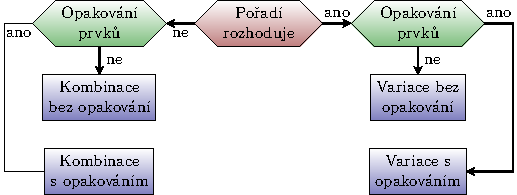
\includegraphics[width=0.7\linewidth]{mai_fig021.pdf}
        \caption{Typy výběrů. \cite[s.~201]{Musilova2009MA1}}
        \label{mai_fig021}
      \end{figure}

      Představuje-li daný výběr například volejbalové družstvo osmi děvčat (šest hráček a dvě 
      náhradnice), které bude reprezentovat v soutěži třídu osmou bé, do níž chodí \num{25} děvčat 
      a \num{18} chlapců, jedná se o výběr \(k — 8\) prvků z počtu \(n = 25\) prvků. Chlapce nelze 
      postavit do družstva volejbalistek. Každý výběr možného družstva bude představovat 
      \emph{kombinaci bez opakování}, neboť pořadí hráček nehraje roli a třeba Aničku Novákovou 
      máme ve třídě jen jednu. Budeme-li však chtít vytvářet z deseti cifer \(0, 1, \ldots, 9\) 
      trojciferná čísla, pak tyto výběry tří prvků z deseti (\(k = 3\), \(n = 10\)) jsou 
      \emph{variacemi s opakováním}. Čísla \num{125}, \num{512}, \num{251}, \num{215}, \num{521} a 
      \num{152} jsou totiž různá, a například \num{222} je také trojciferné číslo. Kombinace s 
      opakováním bychom mohli vytvářet třeba i při výběru různobarevných ponožek ze zásuvky a 
      konečně \emph{variacemi bez opakování} by mohly být dejme tomu trojbarevné signály (\(k = 
      3\)) tvořené trojicemi barevných hadříků vybíraných z \(n\) barev (pro \(n = 3\) třeba zrovna 
      z těch ponožek). Nyní bychom však rádi věděli, jak pro zadané hodnoty \(n\) a \(k\) určit 
      počet všech možných výběrů předepsaného typu. Ukážeme si to na příkladech.

      %---------------------------------------------------------------
      % !TeX spellcheck = cs_CZ
\begin{mdframed}[style=mdexam]
  \begin{example}\label{mai:exam007}
    \textbf{Šance milion}:\newline
    „Znáte nějakou jinou hru, kde můžete denně vyhrát milion?“ Tento nebo jiný, obdobně nepříliš
    vtipný reklamní slogan propaguje v televizi hru, jejímž cílem je uhodnout šestici tažených cifer
    ve správném pořadí. (Hru raději nehrajte, pravděpodobnost výhry je mizivá.) Tah se provádí
    následovně: V každém ze šesti bubnů, očíslovaných pořadovými čísly \num{1} až \num{6}, je
    připraveno deset míčků opatřených ciframi \(0, 1, \ldots, 9\). Z prvního bubnu se náhodně
    vylosuje jedna cifra (deset možností). Poté se náhodně vylosuje jedna cifra z druhého bubnu
    (opět deset možností). Možností vzniku uspořádané dvojice cifer (jedna cifra z prvního a druhá z
    druhého bubnu) je již sto (každou možnost výsledku u prvního bubnu lze kombinovat s každou
    možností výsledku z druhého bubnu). Losování pokračuje u třetího, čtvrtého, pátého a šestého
    bubnu. Celkový počet možností je \num{1e6}, tedy \textbf{milion}. (Šance získat výhru, tedy
    vyhrát milion, je ovšem pouze jedna milióntina, neboť z milionu možností je pouze jedna skutečně
    tažena.) 
  \end{example}
\end{mdframed}
      %---------------------------------------------------------------
      
      Zobecněním předchozího příkladu získáváme vzorec pro počet \textbf{variací s opakováním} 
      \emph{k}-té třídy z \(n\) prvků. Při tahu totiž záleží na pořadí bubnů a každý buben obsahuje 
      všechny cifry. Výsledky tahů z jednotlivých bubnů se tedy mohou opakovat. Pokud by bubnů bylo 
      \(k\) a v každém \(n\) různých cifer, dostali bychom pro \textbf{variace s opakováním 
      \(k\)-té třídy z \(n\) prvků} celkový počet
      \begin{equation}\label{mai:eq007}
        \boxed{V_k' = n^k}\, .
      \end{equation}

      %---------------------------------------------------------------
      % !TeX spellcheck = cs_CZ
\begin{example}\label{mai:exam008}
  \textbf{Modifikovaná šance milion}:\newline
  Představme si hru z předchozího příkladu upravenou takto: K dispozici bude jen jeden buben s 
  ciframi \(0, 1, \ldots, 9\), každá cifra je v bubnu obsažena pouze jednou. Opět máme losovat 
  uspořádanou \textbf{šestici cifer}. Nyní se však jedná o \textbf{variace šesté třídy z deseti 
  prvků bez opakování}. S jediným bubnem musíme totiž provést šest losování, přičemž při každém 
  losování ubude z bubnu jedna cifra. Při prvním tahu je deset možností, při druhém již jen devět, 
  atd., při šestém již pouze pět možností. Celkem je tedy \(10 \cdot 9 \cdots 5 = \num{151200}\) 
  možností.
\end{example}
      %---------------------------------------------------------------
      
      Uvážíme-li, že v předchozím příkladu je \(n = 10\) a \(k = 6\), dostáváme pro \textbf{počet 
      variací bez opakování \(k\)-té třídy z \(n\) prvků} obecný vztah
      \begin{align}
        V_k(n) &= n(n-1)(n-2)\cdots(n-k+1)  \nonumber \\
        \shortintertext{neboli}
        V_k(n) &= \frac{n!}{(n-k)!}\, .    \label{mai:eq008}
      \end{align}
      Poznamenejme, že \(n!\) značí \textbf{faktoriál}, \(n! = n(n — 1)\cdots 3 \cdot 2 \cdot 1\). 
      Pro nulu definujeme \(0! = 1\). Je zřejmé, že při vytváření variací bez opakování musí být 
      \(k\leqq n\). Variace bez opakování \(n\)-té třídy z \(n\) prvků se nazývají 
      \textbf{permutace}. Každá z nich představuje určité uspořádání těchto \(n\) prvků. Platí
      \begin{equation}\label{mai:eq009}
        \boxed{P(n) = V_n(n) = n!}\, .
      \end{equation}
      
      Nyní odvodíme vzorec pro počet \textbf{kombinací \(k\)-té třídy z \(n\) prvků bez opakování}. 
      Již jsme si řekli, že \emph{kombinací} rozumíme takový výběr z celkového počtu \(n\) prvků, 
      který obsahuje určitých \(k\) prvků nezávisle na jejich pořadí. Představme si, že máme k 
      dispozici všechny variace bez opakování \(k\)-té třídy ze zmíněných \(n\) prvků. Vezměme 
      kteroukoli z nich. Soubor všech variací \(k\)-té třídy z \(n\) prvků však obsahuje i další 
      variace, lišící se od té naší jen pořadím prvků. Celkem je takových variací (i s tou první) 
      \(k!\) a z hlediska kombinací představují totéž. Soubor variací se tak rozpadá na podsoubory, 
      z nichž každý obsahuje \(k!\) variací lišících se navzájem pouze pořadím prvků. Každý z 
      těchto podsouborů představuje však jedinou kombinaci. Počet kombinací \(k\)-té třídy z \(n\) 
      prvků bez opakování je tedy
      \begin{equation}\label{mai:eq010}
        \boxed{C(k) = \frac{V_k(n)}{P(k)} = \frac{n!}{(n-k)!\,k!} = 
               \begin{pmatrix}
                n \\
                k
               \end{pmatrix}}\, .
      \end{equation}
      
      Pro odvození vzorce pro \textbf{kombinace s opakováním} použijeme opět příkladu.
      %---------------------------------------------------------------
      % !TeX spellcheck = cs_CZ
\begin{mathexam}{Kuličky v přihrádkách}{exam009}
  Máme kuličky \(n\) různých barev, v každé barvě máme tolik kuliček, kolik bude potřeba. Naším
  úkolem je vytvářet výběry \(k\) kuliček. Na \textbf{pořadí barev nezáleží}, kuliček jedné barvy
  může být ve výběru libovolný počet \(0\leqq s \leqq k\). Výběry budeme vytvářet tak, že budeme
  kuličky dávat do \(n\) přihrádek, z nichž každá bude vyhrazena pro určitou barvu. Pokud tedy v
  daném výběru zrovna nebude třeba modrá kulička, bude přihrádka vyhrazená pro modrou barvu prázdná.
  Budou-li v daném výběru právě tři červené kuličky, budou umístěny v přihrádce vyhrazené pro
  červenou barvu. Vidíme, že pokud konkrétním přihrádkám přisoudíme konkrétní barvy, samotné kuličky
  by již barevné být nemusely, stačily by třeba kuličky skleněné, bezbarvé. Zůstane-li například
  přihrádka pro modrou barvu prázdná, víme, že daný výběr neobsahuje modrou barvu. Budou-li v
  přihrádce pro červenou barvu tři (bezbarvé) kuličky, víme, že daný výběr obsahuje červenou barvu
  třikrát. Příklad takové situace ukazuje následující schéma:
  
  {\centering
    \luafigure[0.9]{mai_fig033.pdf}
    \par}

  Náš úkol můžeme přeformulovat takto: Je třeba rozmístit \(k\) kuliček do \(n\) přihrádek. V každé
  přihrádce může být obecně \(s\) kuliček, kde \(0\leqq s \leqq k\), přitom celkový počet kuliček
  musí být samozřejmě stále \(k\). Můžeme si představit, že \(k\) kuliček máme položených v řadě na
  polici mezi dvěma pevnými stěnami (krajní svislé čáry v předchozím schématu) a různé způsoby
  rozmístění kuliček do přihrádek provádíme přemísťováním pohyblivých přepážek. Kdybychom například
  v předchozím schématu přesunuli druhou svislou čáru, počítáno zleva, až za první kuličku v
  přihrádce na červenou barvu, dostaneme uspořádání, při němž je v přihrádce na modrou barvu jedna
  kulička a v přihrádce na červenou barvu dvě kuličky. Tedy takto:

  {\centering
    \luafigure[0.9]{mai_fig034.pdf}
  \par}

  Mezi dvěma krajními pevnými stěnami máme tedy k dispozici \(k\) pozic pro kuličky a \((n - 1)\)
  pozic pro pohyblivé přepážky. Celkem tedy \((n + k - 1)\) pozic, na které můžeme libovolně
  rozmísťovat \(k\) kuliček a \((n - 1)\) přepážek. Do těchto \((n + k - 1)\) pozic můžeme umístit
  \(k\) kuliček \(C_k'(n)\) způsoby, kde
  \begin{equation}\label{MAI:eq011}
    \boxed{C_k'(n) =  \binom{n + k - 1}{k} = \binom{n + k - 1}{n -1}}\, .
  \end{equation}
  Na zbylé pozice již musíme umístit přepážky. Nebo naopak, nejprve umístíme \((n - 1)\) přepážek a
  potom kuličky. Výsledek je stejný, jak je vidět z předchozího vzorce. Protože jsme vytváření
  kombinací s opakováním \(k\)-té třídy z \(n\) prvků převedli na úlohu o rozmísťování kuliček do
  přihrádek, udává získaný vzorec právě počet takových kombinací. Aby měl vzorec smysl, musí platit
  \(n + k - 1 \geqq k\), tedy \(n \geqq 1\).

  Komu nevyhovuje představa kuliček v přihrádkách a má raději čísla, může uvažovat následovně: Tak
  jako je každé číslo v desítkové soustavě zapsáno pomocí cifer \(0, 1, 2, \ldots , 8, 9\), je k
  jeho zápisu ve dvojkové soustavě potřeba pouze dvou cifer, nuly a jedničky. Představme si nyní
  přepážku jako jedničku a kuličku jako nulu. Náš úkol zjistit počet všech možných způsobů rozdělení
  \(k\) kuliček do \(n\) přihrádek, ohraničených \((n+1)\) přepážkami, můžeme převést na
  ekvivalentní problém: Kolik dokážeme najít čísel, která jsou ve dvojkové soustavě zapsána právě
  \(k\) nulami a \((n + 1)\) jedničkami, požadujeme-li, aby první i poslední cifrou byla jednička?
  Odpověď je jednoduchá. Máme k dispozici \((n+k+1)\) pozic pro cifry. První a poslední pozice jsou
  pevně obsazeny jedničkami, volných pozic je tedy pouze \((n + k - 1)\). Počet všech různých
  způsobů, kterými na \(k\) z těchto pozic můžeme umístit nuly, je roven počtu kombinací \(k\)-té
  třídy z \((n + k - 1)\) prvků. Na zbylé pozice již musíme umístit jedničky. Komplementárně,
  budeme-li hledat počet všech možných způsobů, jak na \((n-1)\) pozic umístit jedničky, dostaneme
  shodný výsledek, v souhlasu se vzorcem (\ref{mai:eq010}).
\end{mathexam}
      %---------------------------------------------------------------
      
      Komu nevyhovuje představa kuliček v přihrádkách a má raději čísla, může uvažovat následovně: 
      Tak jako je každé číslo v desítkové soustavě zapsáno pomocí cifer \(0, 1, 2, \ldots , 8, 9\), 
      je k jeho zápisu ve dvojkové soustavě potřeba pouze dvou cifer, nuly a jedničky. Představme 
      si nyní přepážku jako jedničku a kuličku jako nulu. Náš úkol zjistit počet všech možných 
      způsobů rozdělení \(k\) kuliček do \(n\) přihrádek, ohraničených \((n+1)\) přepážkami, můžeme 
      převést na ekvivalentní problém: Kolik dokážeme najít čísel, která jsou ve dvojkové soustavě 
      zapsána právě \(k\) nulami a \((n + 1)\) jedničkami, požadujeme-li, aby první i poslední 
      cifrou byla jednička? Odpověď je jednoduchá. Máme k dispozici \((n+k+1)\) pozic pro cifry. 
      První a poslední pozice jsou pevně obsazeny jedničkami, volných pozic je tedy pouze \((n + k 
      — 1)\). Počet všech různých způsobů, kterými na \(k\) z těchto pozic můžeme umístit nuly, je 
      roven počtu kombinací \(k\)-té třídy z \((n + k — 1)\) prvků. Na zbylé pozice již musíme 
      umístit jedničky. Komplementárně, budeme-li hledat počet všech možných způsobů, jak na 
      \((n—1)\) pozic umístit jedničky, dostaneme shodný výsledek, v souhlasu se vzorcem 
      (\ref{mai:eq010}).
      
      %---------------------------------------------------------------
      % !TeX spellcheck = cs_CZ
\begin{example}\label{mai:exam010}
  \textbf{Obsazování kvantových stavů}:\newline\small
  Úloha o kuličkách a přihrádkách má přímou aplikaci v \textbf{kvantové fyzice}. Představme si, že 
  fyzikální soustava je tvořena \(k\) částicemi. Každá částice se nachází v určitém stavu, v němž 
  jí můžeme přisoudit fyzikální charakteristiky, které jsou s tímto stavem spojeny (třeba energii, 
  moment hybnosti, apod.). Jednotlivé stavy jsou pak rozlišitelné právě pomocí těchto 
  charakteristik. Dejme tomu, že přípustných stavů je \(n \geqq 1\). Problémem kvantové fyziky je 
  to, že kvantové částice jsou nerozlišitelné. Nepoznáme jednu od druhé. Je to stejné, jako bychom 
  měli \(k\) naprosto stejně vypadajících kuliček, které nemáme nijak očíslovány. Záměna dvou 
  částic (nerozlišitelných kuliček) se nepozná, nevede tedy ke změně stavu fyzikální soustavy. Pro 
  hodnoty fyzikálních charakteristik soustavy jako celku je tedy důležité jen to, kolik částic je v 
  každém z přípustných stavů. Musíme se tedy zajímat o to, kolika způsoby lze našich \(k\) 
  \textbf{nerozlišitelných částic} (kuliček) umístit do \(n\) \textbf{stavů} (přihrádek). Kvantové 
  částice jsou však dvojího druhu, \textbf{fermiony} (například elektrony, neutrony, protony, jádra 
  s lichým počtem nukleonů) a \textbf{bosony} (například fotony, mezony, jádra se sudým počtem 
  nukleonů). Rozdíl mezi nimi je ten, že bosony se „dobře snášejí“, a proto jich může být v jednom 
  stavu i více. 
  \begin{itemize}\addtolength{\itemsep}{-0.5\baselineskip}
    \item Počet možností, jak rozmístit \(k\) \textbf{bosonů} po \(n\) stavech je tedy
          \begin{equation*}
            N_{\text{boson}} = 
              \begin{pmatrix}
                n + k - 1 \\
                    k
               \end{pmatrix}
          \end{equation*}
    \item S \textbf{fermiony} je tomu jinak. \textbf{Pauliho vylučovací princip} jim zakazuje, 
          aby v daném stavu byl více než jeden fermion. Stav může být buď prázdný, nebo obsazen 
          jedním fermionem. V takovém případě musí být \(n \geqq k\) a v každé přihrádce může být 
          nejvýše jedna kulička. Situace tak odpovídá \textbf{kombinacím bez opakování \(k\)-té 
          třídy z \(n\) prvků}, tj.
          \begin{equation*}
            N_{\text{fermion}} = 
              \begin{pmatrix}
                n  \\
                k
              \end{pmatrix}
          \end{equation*}
  \end{itemize}
\normalsize
\end{example}
      %---------------------------------------------------------------
      
      Získané kombinatorické vzorce nyní použijeme při řešení základních úloh o pravděpodobnostech. 
      V každé úloze bude důležité
      \begin{itemize}
        \item definovat jev \(A\), jehož pravděpodobnost počítáme,
        \item určit počet \(N\) případů možných, tj. počet všech možných výsledků pokusu, při 
              kterém sledujeme, zda jev \(A\) nastal či nenastal,
        \item určit počet \(M\) případů příznivých, tj. počet těch výsledků daného pokusu, při 
              kterých jev \(A\) nastal.
      \end{itemize}
      
%} %tikzset
---------------------------------------------------------------------------------------------------
\printbibliography[heading=subbibliography]
\addcontentsline{toc}{section}{Seznam literatury}